\documentclass[14pt]{extbook}
\usepackage{multicol, enumerate, enumitem, hyperref, color, soul, setspace, parskip, fancyhdr} %General Packages
\usepackage{amssymb, amsthm, amsmath, latexsym, units, mathtools} %Math Packages
\everymath{\displaystyle} %All math in Display Style
% Packages with additional options
\usepackage[headsep=0.5cm,headheight=12pt, left=1 in,right= 1 in,top= 1 in,bottom= 1 in]{geometry}
\usepackage[usenames,dvipsnames]{xcolor}
\usepackage{dashrule}  % Package to use the command below to create lines between items
\newcommand{\litem}[1]{\item#1\hspace*{-1cm}\rule{\textwidth}{0.4pt}}
\pagestyle{fancy}
\lhead{Makeup Progress Quiz 2}
\chead{}
\rhead{Version B}
\lfoot{2790-1423}
\cfoot{}
\rfoot{Summer C 2021}
\begin{document}

\begin{enumerate}
\litem{
Solve the linear equation below. Then, choose the interval that contains the solution.\[ \frac{5x + 3}{4} - \frac{7x + 5}{8} = \frac{5x + 4}{6} \]\begin{enumerate}[label=\Alph*.]
\item \( x \in [-13.2, -11.3] \)
\item \( x \in [1.2, 1.8] \)
\item \( x \in [-1.7, -0.9] \)
\item \( x \in [-1, 0.6] \)
\item \( \text{There are no real solutions.} \)

\end{enumerate} }
\litem{
Find the equation of the line described below. Write the linear equation in the form $ y=mx+b $ and choose the intervals that contain $m$ and $b$.\[ \text{Perpendicular to } 3 x + 4 y = 4 \text{ and passing through the point } (-7, 3). \]\begin{enumerate}[label=\Alph*.]
\item \( m \in [0.97, 1.75] \hspace*{3mm} b \in [9, 12] \)
\item \( m \in [-1.67, -0.91] \hspace*{3mm} b \in [-7.33, -5.33] \)
\item \( m \in [0.97, 1.75] \hspace*{3mm} b \in [-19.33, -11.33] \)
\item \( m \in [0.66, 1.09] \hspace*{3mm} b \in [12.33, 15.33] \)
\item \( m \in [0.97, 1.75] \hspace*{3mm} b \in [12.33, 15.33] \)

\end{enumerate} }
\litem{
Write the equation of the line in the graph below in Standard Form $Ax+By=C$. Then, choose the intervals that contain $A, B, \text{ and } C$.
\begin{center}
    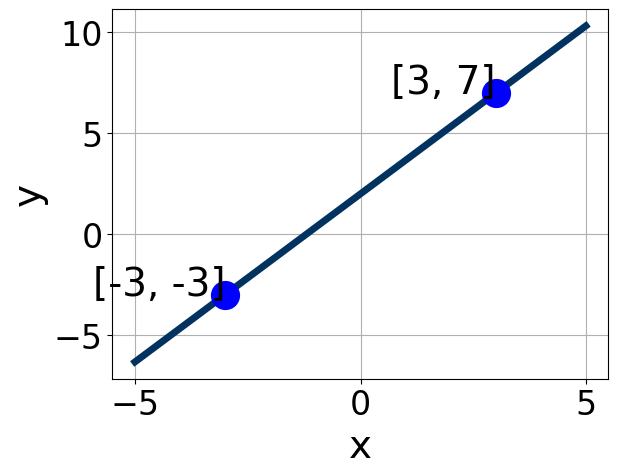
\includegraphics[width=0.5\textwidth]{../Figures/linearGraphToStandardCopyB.png}
\end{center}
\begin{enumerate}[label=\Alph*.]
\item \( A \in [3.8, 6.1], \hspace{3mm} B \in [1.6, 3.2], \text{ and } \hspace{3mm} C \in [5.2, 6.9] \)
\item \( A \in [-6, -4.7], \hspace{3mm} B \in [1.6, 3.2], \text{ and } \hspace{3mm} C \in [5.2, 6.9] \)
\item \( A \in [-2.8, -1.3], \hspace{3mm} B \in [-1.96, 0.04], \text{ and } \hspace{3mm} C \in [-5.7, -1] \)
\item \( A \in [-2.8, -1.3], \hspace{3mm} B \in [-0.43, 1.42], \text{ and } \hspace{3mm} C \in [1.2, 3.9] \)
\item \( A \in [3.8, 6.1], \hspace{3mm} B \in [-5.33, -1.85], \text{ and } \hspace{3mm} C \in [-7.2, -4.8] \)

\end{enumerate} }
\litem{
First, find the equation of the line containing the two points below. Then, write the equation in the form $ y=mx+b $ and choose the intervals that contain $m$ and $b$.\[ (-11, 8) \text{ and } (2, 2) \]\begin{enumerate}[label=\Alph*.]
\item \( m \in [-1.54, 0.12] \hspace*{3mm} b \in [-4.35, -2.3] \)
\item \( m \in [-1.54, 0.12] \hspace*{3mm} b \in [18.24, 19.45] \)
\item \( m \in [-1.54, 0.12] \hspace*{3mm} b \in [-0.88, 0.95] \)
\item \( m \in [-1.54, 0.12] \hspace*{3mm} b \in [2.36, 3.43] \)
\item \( m \in [-0.35, 1.07] \hspace*{3mm} b \in [1.04, 1.74] \)

\end{enumerate} }
\litem{
Solve the equation below. Then, choose the interval that contains the solution.\[ -3(12x + 17) = -4(18x -7) \]\begin{enumerate}[label=\Alph*.]
\item \( x \in [-0.46, 0.59] \)
\item \( x \in [-1.71, -0.3] \)
\item \( x \in [0.58, 1.15] \)
\item \( x \in [2.03, 2.62] \)
\item \( \text{There are no real solutions.} \)

\end{enumerate} }
\litem{
First, find the equation of the line containing the two points below. Then, write the equation in the form $ y=mx+b $ and choose the intervals that contain $m$ and $b$.\[ (11, 2) \text{ and } (5, -3) \]\begin{enumerate}[label=\Alph*.]
\item \( m \in [-0.2, 1.7] \hspace*{3mm} b \in [-8.08, -7.75] \)
\item \( m \in [-0.2, 1.7] \hspace*{3mm} b \in [6.77, 8.18] \)
\item \( m \in [-0.2, 1.7] \hspace*{3mm} b \in [-9.51, -8.91] \)
\item \( m \in [-0.2, 1.7] \hspace*{3mm} b \in [-7.19, -6.58] \)
\item \( m \in [-3.5, -0.4] \hspace*{3mm} b \in [0.75, 1.58] \)

\end{enumerate} }
\litem{
Solve the linear equation below. Then, choose the interval that contains the solution.\[ \frac{5x -3}{6} - \frac{7x + 4}{3} = \frac{-5x -5}{4} \]\begin{enumerate}[label=\Alph*.]
\item \( x \in [7.5, 9.7] \)
\item \( x \in [-1, 0.4] \)
\item \( x \in [-8.8, -6.4] \)
\item \( x \in [-2.5, -1.5] \)
\item \( \text{There are no real solutions.} \)

\end{enumerate} }
\litem{
Find the equation of the line described below. Write the linear equation in the form $ y=mx+b $ and choose the intervals that contain $m$ and $b$.\[ \text{Perpendicular to } 7 x + 3 y = 8 \text{ and passing through the point } (-8, 2). \]\begin{enumerate}[label=\Alph*.]
\item \( m \in [2.15, 2.99] \hspace*{3mm} b \in [4.8, 6.6] \)
\item \( m \in [0.34, 0.8] \hspace*{3mm} b \in [8.3, 12.4] \)
\item \( m \in [0.34, 0.8] \hspace*{3mm} b \in [-5.9, -3] \)
\item \( m \in [0.34, 0.8] \hspace*{3mm} b \in [4.8, 6.6] \)
\item \( m \in [-0.91, -0.08] \hspace*{3mm} b \in [-1.6, -0.9] \)

\end{enumerate} }
\litem{
Write the equation of the line in the graph below in Standard Form $Ax+By=C$. Then, choose the intervals that contain $A, B, \text{ and } C$.
\begin{center}
    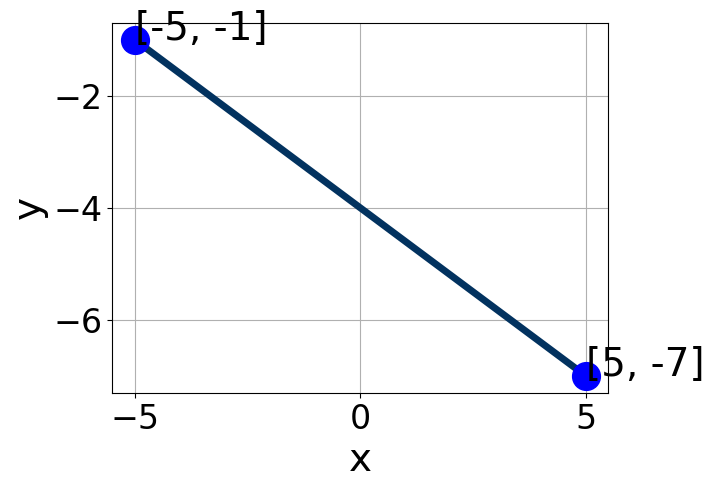
\includegraphics[width=0.5\textwidth]{../Figures/linearGraphToStandardB.png}
\end{center}
\begin{enumerate}[label=\Alph*.]
\item \( A \in [-0.2, 2.6], \hspace{3mm} B \in [0.71, 1.37], \text{ and } \hspace{3mm} C \in [-8, -1] \)
\item \( A \in [1.9, 5.1], \hspace{3mm} B \in [-5.68, -4.25], \text{ and } \hspace{3mm} C \in [20, 25] \)
\item \( A \in [-0.2, 2.6], \hspace{3mm} B \in [-1.54, 0.53], \text{ and } \hspace{3mm} C \in [4, 9] \)
\item \( A \in [-3.8, -2.3], \hspace{3mm} B \in [-5.68, -4.25], \text{ and } \hspace{3mm} C \in [20, 25] \)
\item \( A \in [1.9, 5.1], \hspace{3mm} B \in [4.46, 6.38], \text{ and } \hspace{3mm} C \in [-21, -17] \)

\end{enumerate} }
\litem{
Solve the equation below. Then, choose the interval that contains the solution.\[ -13(15x -11) = -4(-6x + 5) \]\begin{enumerate}[label=\Alph*.]
\item \( x \in [0.53, 0.57] \)
\item \( x \in [0.74, 0.76] \)
\item \( x \in [-0.59, -0.55] \)
\item \( x \in [0.71, 0.74] \)
\item \( \text{There are no real solutions.} \)

\end{enumerate} }
\end{enumerate}

\end{document}